\documentclass[10pt, aspectratio=169]{beamer}

\usetheme[progressbar=frametitle]{metropolis}
\usepackage{appendixnumberbeamer}

\usepackage{booktabs}
\usepackage[scale=2]{ccicons}

\usepackage{pgfplots}
\usepgfplotslibrary{dateplot}
\definecolor{customgrey}{RGB}{240,240,240} % Light grey
\definecolor{customorange}{RGB}{255,102,0} % Orange
\usepackage[most]{tcolorbox}
\usepackage{lmodern}
\usepackage{listings}
\usepackage{xcolor}
\usepackage{amsmath}
\usepackage{animate}
\usepackage{svg}

\usepackage[
    backend=biber, 
    style=apa,
    hyperref=true
    ]{biblatex}
\addbibresource{latex/references.bib}

\definecolor{lightgray}{gray}{0.95}

\newtcblisting{promptblock}{
  colback=lightgray,
  colframe=,
  listing only,
  listing options={
    basicstyle=\ttfamily\small,
    breaklines=true,
    columns=fullflexible,
    keepspaces=true
  },
  title=,
  fonttitle=\bfseries,
  enhanced,
  boxrule=0.8pt,
  sharp corners,
  left=2mm,
  right=2mm,
  top=1mm,
  bottom=1mm
}
\setbeamercolor{block title alerted}{fg=white,bg=customorange}
\setbeamercolor{block body alerted}{fg=black,bg=customgrey}
\setbeamerfont{block title alerted}{series=\bfseries}
\setbeamerfont{block body alerted}{}
\usepackage{xspace}
\newcommand{\themename}{\textbf{\textsc{metropolis}}\xspace}


\title{Folk Around and Find Out}
\subtitle{Algorithmic Collusion and the Limits of Coordination}

% \date{\today}
\date{}
\author{Lucia Sauer, Julian Romero \& Moritz Peist }
\institute{Barcelona School of Economics}
%\logo{\includesvg[width=0.2\linewidth]{latex/imgs/BSE Barcelona Graduate School of Economics.svg}}
% \titlegraphic{\hfill\includegraphics[height=1.5cm]{logo.pdf}}

\begin{document}

\maketitle

\begin{frame}{Motivation}
\begin{figure}
        \centering
        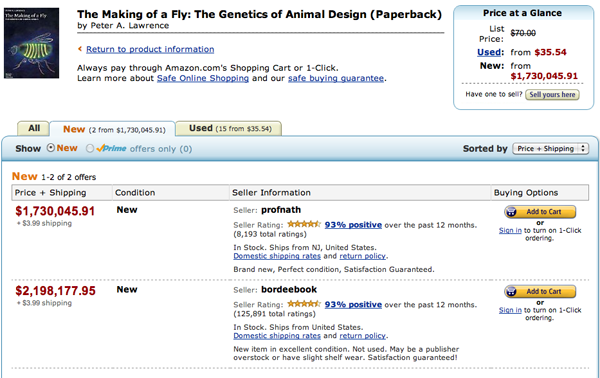
\includegraphics[width=0.7\linewidth]{latex/slides_pricing_collusion/imgs/the_making_of_a_fly.png}
        \caption{Two pricing algorithms made a biology textbook cost \$23 million. As Margrethe Vestager put it: someone finally noticed… and adjusted it manually.}
        \label{fig:rep_org}
    \end{figure}  
\end{frame}


\begin{frame}{Background on AP Collusion}

    
\end{frame}


\begin{frame}{LLM for pricing?}

    
\end{frame}


\begin{frame}{Research question}

\end{frame}

\section{Experimental Set up}

\begin{frame}[fragile]{}
We replicate this paper using Open Source Models, where \textbf{Mistral LLMs show agentic pricing capabilities and collusive behavior}.


\end{frame}


\subsection{}


\begin{frame}[fragile]{Our Implementation}
\begin{figure}
    \centering
    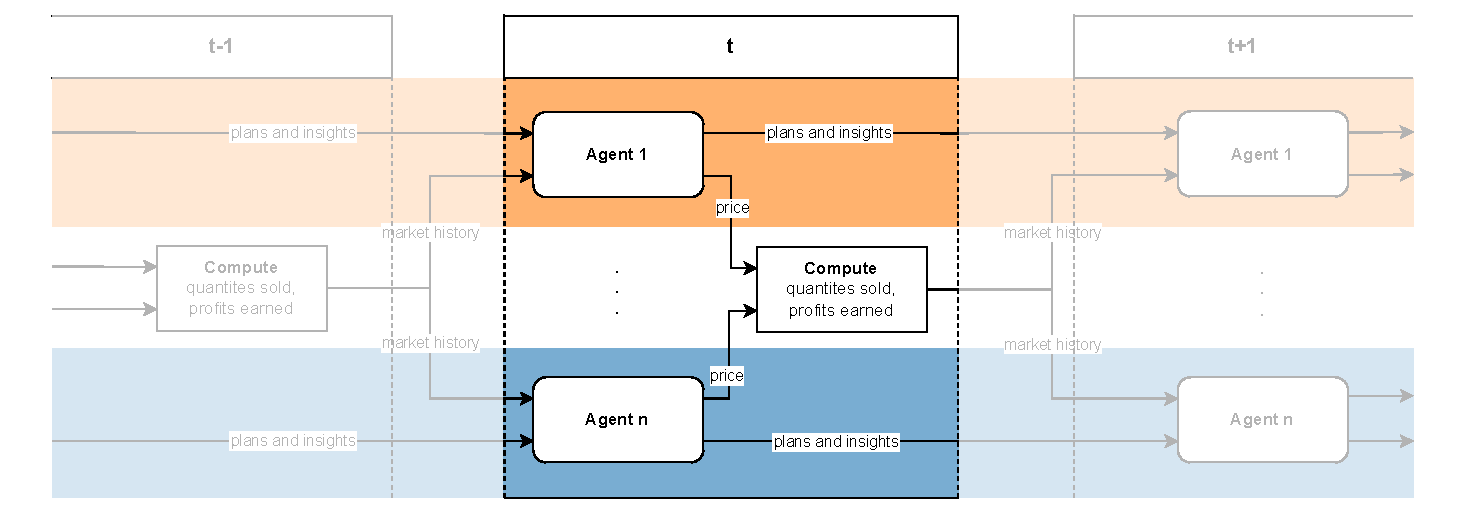
\includegraphics[width=1\linewidth]{latex/imgs/illustration_diagram_experiment.pdf}
    \caption{}
    \label{fig:enter-label}
\end{figure}
  
\end{frame}

\begin{frame}[fragile]{Pricing Agents}
\begin{columns}[T,onlytextwidth] % Top-aligned columns
    \column{0.48\textwidth}
    \textbf{Prompt Structure:}
    \begin{enumerate}[]
        \item \textbf{Prompt prefix:} 
        \item \textbf{Cost info:} 
        \item \textbf{Market history:}
        \item \textbf{Planning context:}
        \item \textbf{Output instructions:}
    \end{enumerate}

    \column{0.52\textwidth}
    \begin{promptblock}
# Prompt Prefix
You are a pricing agent aiming to maximize long-term profit.

# Cost Information
Current marginal cost: c_t^i = 3.45


    \end{promptblock}
\end{columns}
\end{frame}

\begin{frame}[fragile]{Demand function}
\begin{itemize}
    \item \textcite{calvano_artificial_2020} Demand Function
    $$
q_i = \beta \cdot \frac{e^{\frac{a_i - p_i/\alpha}{\mu}}}{\sum_{j=1}^{n} e^{\frac{a_j - p_j/\alpha}{\mu}} + e^{\frac{a_0}{\mu}}}
$$
\begin{itemize}
    \item $a_1, a_2, \ldots, a_n$: product-specific attributes (differentiation), with $a_0$: baseline demand intercept.
    \item $\alpha=1, \beta=100$: scaling parameters. $\alpha$ affects currency unit, $\beta$ quantity scaling factor.
    \item $a_0 = 0$, $\mu = 0.25$, all from Calvano et al. (2020b).
\end{itemize}
    \item Focus on markup, taking advantage of the real market structure
    \begin{itemize}
        \item Inelastic demand (people need gas regardless)
        \item Sticky market shares due to location/convenience
        \item Competition primarily on margins, not volume
    \end{itemize}
\end{itemize}
  
\end{frame}



% Uncomment this to increase performance 
%\begin{frame}{What's going on?}
%    \begin{figure}
%        \centering
%        \animategraphics[controls, 
%            autoplay, % Starts playing immediately
%            autoresume, % Resumes after page focus returns
%            autopause, % Pauses when page loses focus
%            width=0.7\linewidth]{10}{latex/slides_pricing_collusion/imgs/beamer_frames/frame_}{000}{299}
%        \caption{300 period run---P1, 5 firms }
%        \label{fig:run}
%    \end{figure}
%\end{frame}



%\appendix

%\begin{frame}[fragile]{Backup slides}
% -
%\end{frame}

%\begin{frame}[allowframebreaks]{References}

%  \bibliography{demo}
%  \bibliographystyle{abbrv}

%\end{frame}

\end{document}
